\documentclass[twocolumn,a4paper]{article}
\title{\textbf{IN4391 Distributed Computing Systems \\ Lab Exercise A}}
\author{Anass Drif(4030532) \and Matthijs van Dorth(1265911)}

\usepackage{amsmath}
\usepackage{epsfig}

\begin{document}
\maketitle


\begin{abstract}
In this article we explain the extensions we made to the Virtual Grid Simulator. With these extensions the Grid Simulator is now a distributed application that can run across multiple different machines. Because of the distributed nature of the application it is now possible to scale the application in using even more and larger virtual clusters. The distributed setup enables a more fault resilient application since the failing of one or more components doesn't necessarily mean the application will fail. How both the scalability and fault tolerance are improved is explained in the following article as well as how we did some initial testing in a distributed environment.
\end{abstract}

\section{Introduction}
As today's cluster grow larger and and larger, spanning multiple organizations, sometimes even on multiple continents, these clusters get harder and harder to manage. A gridscheduler is a machine that assigns jobs to different nodes on a cluster. With a large number of clusters, a gridscheduler as a single machine is a bottleneck for the system. The system is not scalable and has a single point-of-failure. To overcome these problems we provide a distributed solution, where multiple gridschedulers work together to manage the clusters, and deal with failing clusters or gridschedulers.

\section{Single machine solution}
The initial Virtual Grid Simulator consisted of a single GridScheduler (GS) that managed multiple clusters. Each cluster had a single Resource Manager (RM) that is responsible for the scheduling of jobs on individual nodes in the cluster. Jobs are offered to this RM and it has the option to either accept a job for execution on its own cluster or to offload it to the GS when the cluster jobqueue exceeded a certain threshold. When a job is offloaded to the gridscheduler, he offloads it to the RM of a cluster that is the least loaded. This information is maintained by the gridscheduler as he offloads jobs to the RMs.

\begin{figure}
	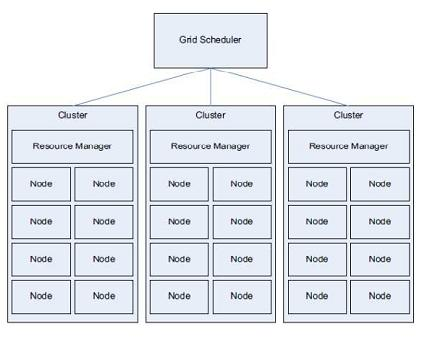
\includegraphics[scale=0.7]{singleGS.jpg}
	\caption{Original VGS with single Gridscheduler.}
\end{figure}

\section{Distributed solution}
A distributed solution consists of having multiple gridschedulers that can be contacted by the RMs. Each gridscheduler maintains the load of each cluster in a hashmap, this way they can balance the load between the clusters. Load-balancing is very important, otherwise some clusters may wear faster than others. But this of course introduces some challenges, regarding maintaining the same view of the clusters, and how to deal with leaving and joining gridschedulers. In the next two sections, we will elaborate on how we dealt with the replication and consistency problem, and how we made the system fault-tolerant.

\begin{figure}
	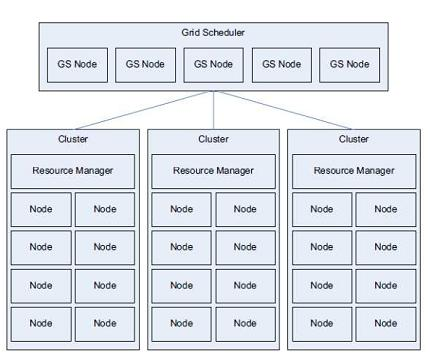
\includegraphics[scale=0.7]{distributedGS.jpg}
	\caption{Distributed solution with multiple Gridschedulers.}
\end{figure}

\subsection{Initialization}
Each Resource Manager is initialized with one random Gridscheduler that is active at the moment the Resource Manager comes online. It then contacts this Gridscheduler to inform it about its existence. The Gridscheduler then sends back an acknowledgment and forwards this info to the other Gridschedulers who upon receiving also send an acknowledgment to the Resource Manager.

\subsection{Replication and consistency}
We implemented a very strict, and simple, consistency mechanism regarding the load of the clusters. Whenever a gridscheduler offloads a job to a cluster, it informs all gridschedulers about this event. It is a very simple mechanism at the cost of a lot of message overhead. We tried to relieve this drawback a little bit, by organizing the nodes in a (bidirectional) ring structure, for a simple communication mechanism, that also divides the communication overhead over all nodes. One might argue that this still can become a very large ring with a large number of nodes in the system. We also designed an optimization for that: bisecting the ring structure in almost equal halves by sending a multicast message in both directions, until they meet somewhere in the middle (influenced by message delay).

\subsection{Fault tolerance}
We designed a fault tolerance mechanism, that utilizes a mesh structure in the node topology to reconstruct the ring in case of node failures by use of gossiping. This is achieved by maintaining a list of known peers. We however only implemented a solution for single node failures (because of time distress caused by exams), which assumes the ring has two broken links caused by the node that failed, and tries to fix that by sending a message in the opposite direction.

\subsection{Failure detection}
A gridscheduler node failure can be detected either by another gridscheduler or by a resource manager of a cluster.
When a resource manager offloads a job to a gridscheduler, it waits for an acknowledgment (asynchronously) for 2 seconds, and if it didn't receive a reply, it removes the gridscheduler from its list of gridschedulers, and retries with another one including in that message the failure of a gridscheduler. The gridscheduler that gets contacted with a Retry message, first informs all clusters that the gridscheduler, or gridschedulers in case it is a double retry, is down. Then it informs the gridschedulers, who immediately go into maintenance mode. When a gridscheduler is in maintenance mode, jobs keep getting received by the clusters, but it does not offload jobs to clusters until the control structure is rebuilt. The two nodes who lost a neighbor both send a message to the other neighbor through the broken ring (assumed there are no other failures). They check whose id is bigger, and that node send a message through the ring announcing the end of maintenance.

Implemented:
\begin{itemize}
	\item (Bidirectional) Ring structure for messaging (communication load divided over all nodes).
	\item Ring reconstruction for single node failure.
	\item Acknowledgments for sending jobs from Cluster to GridScheduler
	\item Loadbalancing clusters requires consistent view of clusters free slots by gridschedulers: strict consistency, every change in a cluster by a gridscheduler, is sent through the ring to inform all other gridschedulers about it
\end{itemize}

Designbed but not implemented:
\begin{itemize}
	\item Mesh structure utilized for ring reconstruction at node failure, achieved by maintaining list of known peers and gossiping
	\item With n nodes, ring of size n, and a k-connected graph (mesh) for ring reconstruction, maintained by a list of k known peers
	\item Acknowledgments between gridscheduler communication
	\item Load balancing jobqueue gridschedulers
	\item Optimizing ring traffic, by bisecting of the ring: send message in both ways, until they meet around half way the ring
\end{itemize}

\subsection{Gridscheduler selection}
The RecourceManager of each cluster offloads a job to one gridscheduler from its list of gridschedulers, obtained at initialization. This selection can be done in a random, or round-robin fashion. We implemented a random selection mechanism. One might consider the round-robin approach, to achieve better load balancing for the job queues of the gridschedulers. We also implemented a load balancing mechanism for the job queues of the gridschedulers, where each node regularly forwards information about its job queue to some destination in the ring structure. Upon receiving this information, a node can check whether the amount of waiting jobs in its queue is at least one order of magnitude higher than of the sending node. If that is so half of the jobs are offloaded to that gridscheduler.


\subsection{Scalability}
Due to the fact that a single GridScheduler can only handle a few clusters, the basic application wasn't very scalable. To be able to manage many clusters, multiple GridSchedulers are needed. We implemented a  GridSchedulerNode that could be deployed on different machines and when working together is able to manage many clusters. Each GridSchedulerNode has a Queue that consists of Jobs that have not finished yet. Each gridscheduler is responsible for the execution of the jobs that are in its Queue. To be able to scale well, all the nodes need to have about the same amount of jobs in its Queue. It is therefore important that all the nodes know what the load is in each node. This is done by passing controlmessages around which contain the load of the nodes. Gridschedulers can offload jobs to other gridschedulers when it passes a certain threshold when it currently has too many jobs waiting. Using this technique we make sure that all the nodes have more or less the same load and this should scale the application in a correct way.

\subsection{Fault Tolerance}
Unfortunately the nodes in the system are not completely resilient against faults, or failures. A node can suddenly crash and loose all of the contents of its Queue. Because you want all jobs sent to the system will be returned when they are finished the jobs need to be backed up somewhere in case a node breaks down. The solution here is to backup all jobs on another node and distribute this backup to all other nodes when a node has failed. The new problem now is, how to detect when a node has crashed? Our solution is to give the responsibility of detecting whether or not a node is crashed to the original upstream and downstream of the node. If both these nodes agree that the node between them has crashed, they will broadcast the fact that this node is no longer available and make a new connection between them so that the bidirectional ring is connected again.

\subsection{Bonus Features}
Besides the scalability and the fault tolerance, we did some additional work to improve this system. Because we think the solutions found in this study may benefit other people as well that face similar problems in fault tolerance or scalability. Therefore the complete source code for the Distributed Grid Scheduler is open source and can be found on GitHub [https://github.com/IN4391/IN4391-1].

\begin{table*}
\begin{tabular}{ |l|l| }
  \hline
  Initialize RMI & Register with rmiregistry \\
  \hline
  Initialize gridschedulers: & send(RequestGSes, random\_gs) \\
  \hline
  OnMessageReceived: & AddJob $\rightarrow$ jobQueue.add(job) \\
  & RequestLoad $\rightarrow$ send(ReplyLoad, requester) \\
  & ReplyGS $\rightarrow$ gridschedulers.add(gs) \\
  & SpawnJob (jobQueue full) $\rightarrow$ send(AddJob, random\_gs); startTimer() \\
  & SpawnJob (jobQueue not full) $\rightarrow$ jobQueue.add(job) \\
  & Roger $\rightarrow$ stopTimer() \\
  & GSDown $\rightarrow$  gridschedulers.remove(gs) \\
  & JoiningGS $\rightarrow$ send(ResourceManagerJoin, gs) \\
  \hline
\end{tabular}
\caption{ResourceManager intialization and message received function.}
\end{table*}

\begin{table*}
\begin{tabular}{ |l|l| }
  \hline
  Initialize RMI & Register with rmiregistry \\
  \hline
  run: & for each ResourceManager rm\\
  & send(RequestLoad, rm) \\
  & for each Job j\\
  & send(AddJob, j)\\
  & leastLoadedRM++\\
  & informOthers()\\
  \hline
  OnMessageReceived: & AddJob $\rightarrow$ jobQueue.add(job); send(Roger, sender) \\
  & RequestGSes $\rightarrow$ rmLoad.put(url); send(ReplyGS, sender); send(ForwardRM, downstream) \\
  & ForwardRM $\rightarrow$ rmLoad.put(url); send(ReplyGS, sender); send(ForwardRM, downstream) \\
  & ReplyLoad $\rightarrow$ rmLoad.put(url) \\
  & UpdateView $\rightarrow$ rmLoad.put(url); send(UpdateView, downstream) \\
  & Retry $\rightarrow$ send(Roger, sender); nodeLeft(gs) \\
  & CrasedGS $\rightarrow$  send(NeighborRequest) $\|$ send(CrashedGS) \\
  & NeighborRequest $\rightarrow$ send(NeighborRequest) $\|$ down or upstream = gs  \\
  & MaintenanceDone $\rightarrow$ maintenance = false; send(MaintenanceDone, downstream)\\
  \hline
\end{tabular}
\caption{GridScheduler polling loop and message received function.}
\end{table*}

\section{Testing}
Simple tests were performed to test the separate mechanisms for fault-tolerance, for example by letting a gridscheduler shut down after some time. What is interesting to measure when this event takes place, is how long it takes for the system to reconstruct its ring structure. Unfortunately even with a large number of gridschedulers this is a negligible amount of time. Since the asynchronous messaging between the clusters and gridschedulers remains intact even when in maintenance mode, a slight peak in the job queues is noticeable.

\section{Experimental Setup}
To see how the improved version of the gridscheduler performed, we conducted a few experiments on the DAS supercomputer located at the TU Delft [note]. Jobs where simulated on different clusters having a variable time between 4 and 12 seconds. The jobs were send to the resourcemanagers at different rates to see how they performed. We used different amounts of Schedulers to see how different they perform and to estimate how well this solution scales.
% - explain amount nodes
% - explain what is on each node
% - setup of gridschedulers
% - getting to 100.000 clusternodes

\section{Results}
After extensive testing we came to the following results...

\section{Discussion and Future work}
The question is how well this will work when the nodes are in different parts of the world. In this experiment we did the test on only one single cluster where the different nodes are close to each other and have a low latency between them. Also due to time constraints the jobs where relatively small, both in size and in time before completion. In a more realistic world the jobs are considerable longer and take a longer time to transit. More realistic testing should be done in order to test how well this works when the schedulers are truly distributed. This wasn't our main goal in this setup in which we where only showing this is a viable option.
During the building of this application we faced different challenges. First thing was that we had to think of how different nodes should communicate with each other, thus designing a new protocol for communication with the nodes. Another challenge was the need for testing this on the DAS-cluster. The DAS-cluster has a particular way of working with nodes that we have to work with. It was quite a challenge to find out how to work with the DAS-cluster as there wasn't any lot of documentation available on how to work with RMI on the DAS-cluster.

\section{Conclusion}
We showed that it is possible to create a distributed scheduler, that is both scalable and fault tolerant. This can be done when the nodes communicate with each other using different message types. The passing around of messages ensures that different nodes know what to do. The specifications of these messages are very important so that all nodes understand each other.
%As a result we where able to manage 100.000 nodes at once using this distributed application.

\end{document}
